\documentclass{article}
\usepackage{graphicx} % Required for inserting images
\usepackage{hyperref}     % Per i link
\usepackage{array}        % Per tabelle con allineamento personalizzato
\usepackage{longtable}    % Per tabelle lunghe e ordinate
\usepackage{listings}    % Pacchetto per il codice
\usepackage{xcolor}      % Per la colorazione del codice
\usepackage{float}   

\lstset{
    language=Python,
    basicstyle=\ttfamily\small,  % Stile del testo
    keywordstyle=\color{blue},   % Colore delle parole chiave
    stringstyle=\color{red},     % Colore delle stringhe
    commentstyle=\color{gray},   % Colore dei commenti
    frame=single,                % Cornice intorno al codice
    numbers=left,                % Numeri di riga a sinistra
    numberstyle=\tiny\color{gray}
}

\title{Algorithms and Data Structures Project \\ \large A Comparative Analysis of Sorting Algorithms}
\author{Federico Del Pup \\
Luigi Pascu \\
Matteo Passador \\
Stefano Toneguzzo
}
\date{Maggio 2025}

\begin{document}

\maketitle

\section*{Contents}
\begin{enumerate}
\item \hyperref[sec:intro]{Introduction and Project Purpose}
\item \hyperref[sec:ling]{Project Organization}
\item \hyperref[sec:grafici]{Analysis of Average Case Scenarios}
\item \hyperref[sec:peggiori]{Analysis of Worst Case Scenarios}
\item \hyperref[sec:partecipanti]{Project Contributors}
\end{enumerate}

\label{sec:intro}

\section{Introduction and Project Purpose}
The purpose of the laboratory project is to design, implement, and analyze sorting algorithms. In particular, the project requires:
\begin{itemize}
\item the correct implementation of four sorting algorithms for arrays of integers, three fixed by the instructor (Quicksort, Countingsort and Quicksort 3-way) and one chosen by the group (Mergesort)
\item the experimental measurement of average execution times as a function of the array size \emph{n} and the range \emph{m} of the integers composing the array
\item the production of comparative charts that show the performance of the algorithms with respect to the execution time \emph{t} based on the two chosen parameters
\item the writing of a technical report in which implementation choices are discussed and the empirical complexity observed is analyzed
\end{itemize}
The final goal is to correctly evaluate the performance of the algorithms, noting their positive characteristics and drawbacks.

\label{sec:ling}
\section{Project Organization}
\subsection*{Language Choice}
The reason for choosing Python lies in several favorable characteristics of the language: being a \textbf{high-level language} has allowed for rapid development of the code without compromising clarity and management.
Moreover, Python offers a wide range of libraries and integrated tools useful for the project. In particular, the \emph{time} library has enabled precise measurements of execution times using the \emph{perf\_counter()} function, while libraries such as \emph{matplotlib} and \emph{numpy} have facilitated the visualization and analysis of the results obtained through \textbf{comparative charts}.

\subsection*{Choice of the Fourth Algorithm}
As the fourth algorithm to analyze, Mergesort was chosen for its guaranteed efficiency in all cases, with complexity $\Theta(n \log (n))$ and sorting stability, which make it a good comparison point with the other required algorithms.

\subsection*{Tools and Development Environment}
To better coordinate project development, a shared file was created on \textbf{Google Colab}. This collaborative environment allowed all group members to work simultaneously on the code, make real-time modifications, and run tests on algorithms dedicated to chart generation.
The code was initially developed in \textbf{separate modules}, each dedicated to a specific functionality. Subsequently, the various components were integrated into a single coherent and functional solution.
For chart generation, we used an \emph{Acer Predator Helios NEO 16}, with \textbf{Intel i9 14900HX CPU} and \textbf{16GB RAM}, using the \textbf{Visual Studio Code} development environment.
Finally, the report was written in LaTeX on \textbf{Overleaf}.

\section{Analysis of Graphs in Average Case Scenarios}
\label{sec:grafici}
\subsection*{Sample Collection}
To generate the graphs, the examined interval was divided into 100 samples. Rather than using a uniform distribution, a \textbf{geometric series} was chosen that starts from the minimum value and gradually increases to the maximum. This approach allows for a \textbf{higher density} of points in the lower part of the range, where differences between algorithms are often more significant.
For each of these 100 samples, a test was conducted: 1000 independent runs of each algorithm were executed.
In each run, a new array with random values was generated.
For every algorithm, the execution time was measured net of array initialization time.
Then the average of the obtained times was calculated.
This methodology allowed us to obtain reliable and significant data, reducing the influence of random factors and focusing on the actual performance of the sorting algorithms.

\subsection*{Variable Array Size}

\begin{figure}[H]
    \centering
    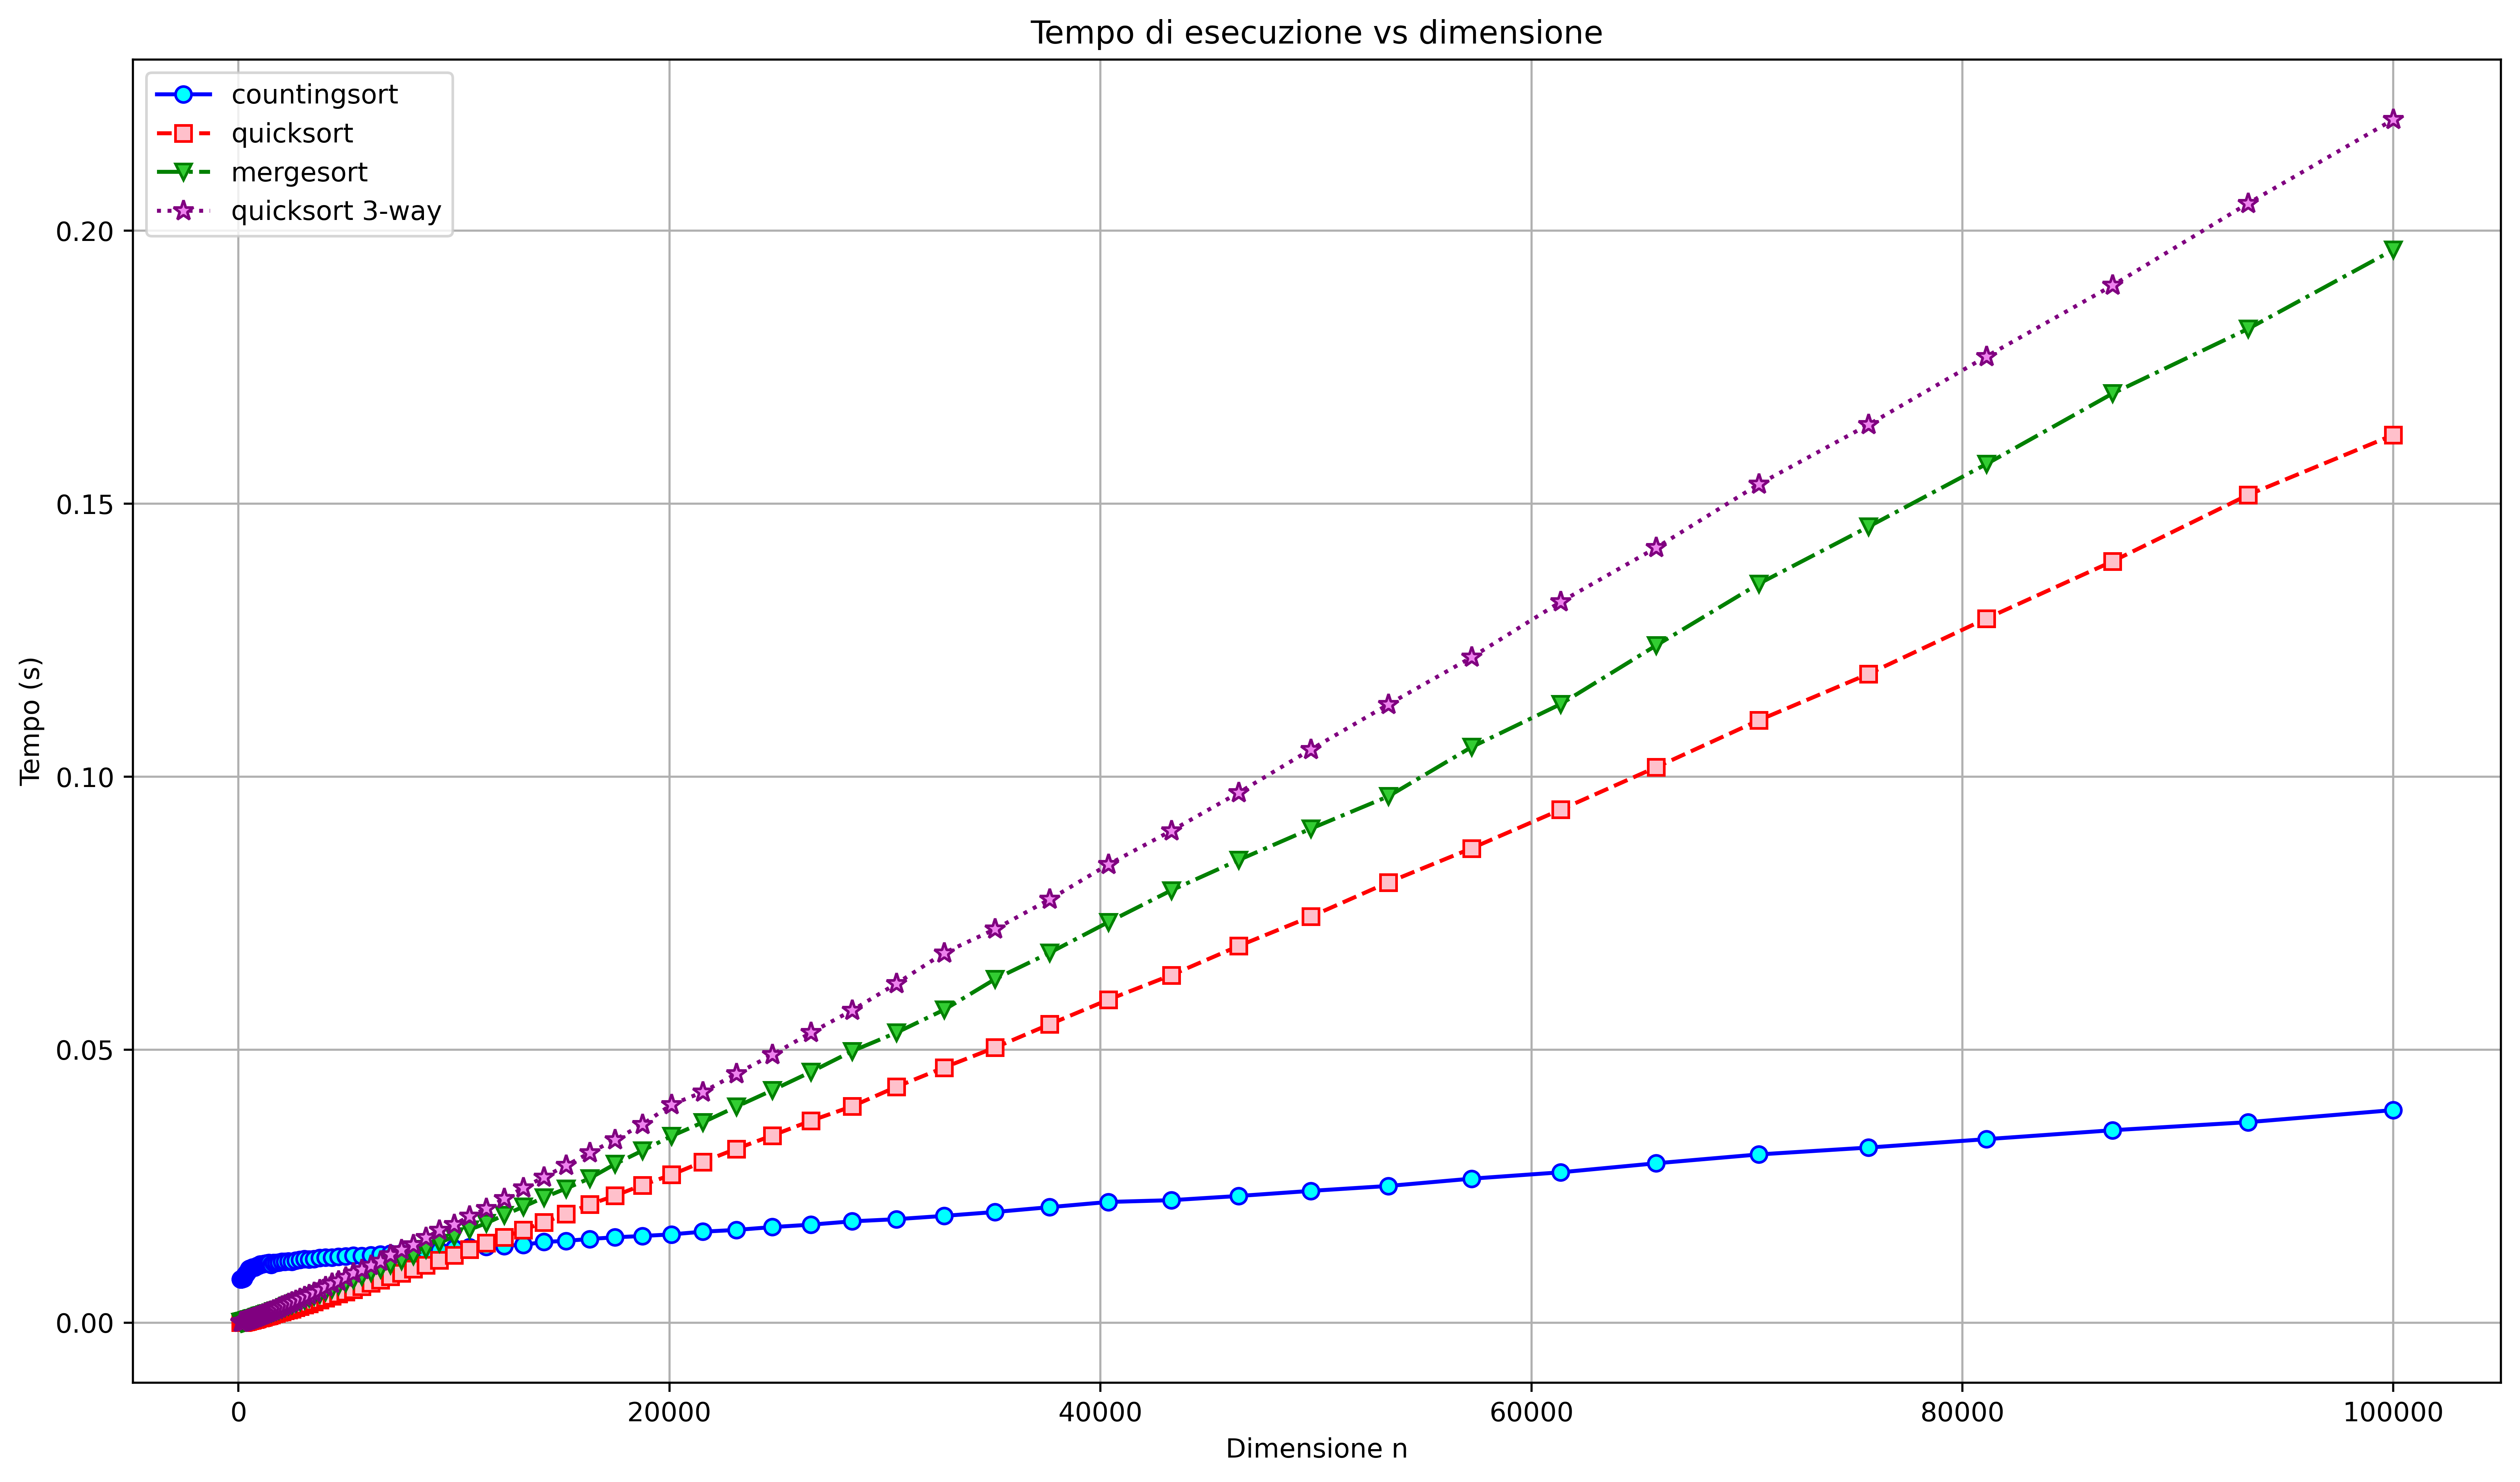
\includegraphics[width=0.95\textwidth]{Casi medi/n.png}
    \caption{Graph as a function of array size \emph{n}}
    \label{fig:n}
\end{figure}
\begin{figure}[H]
    \centering
    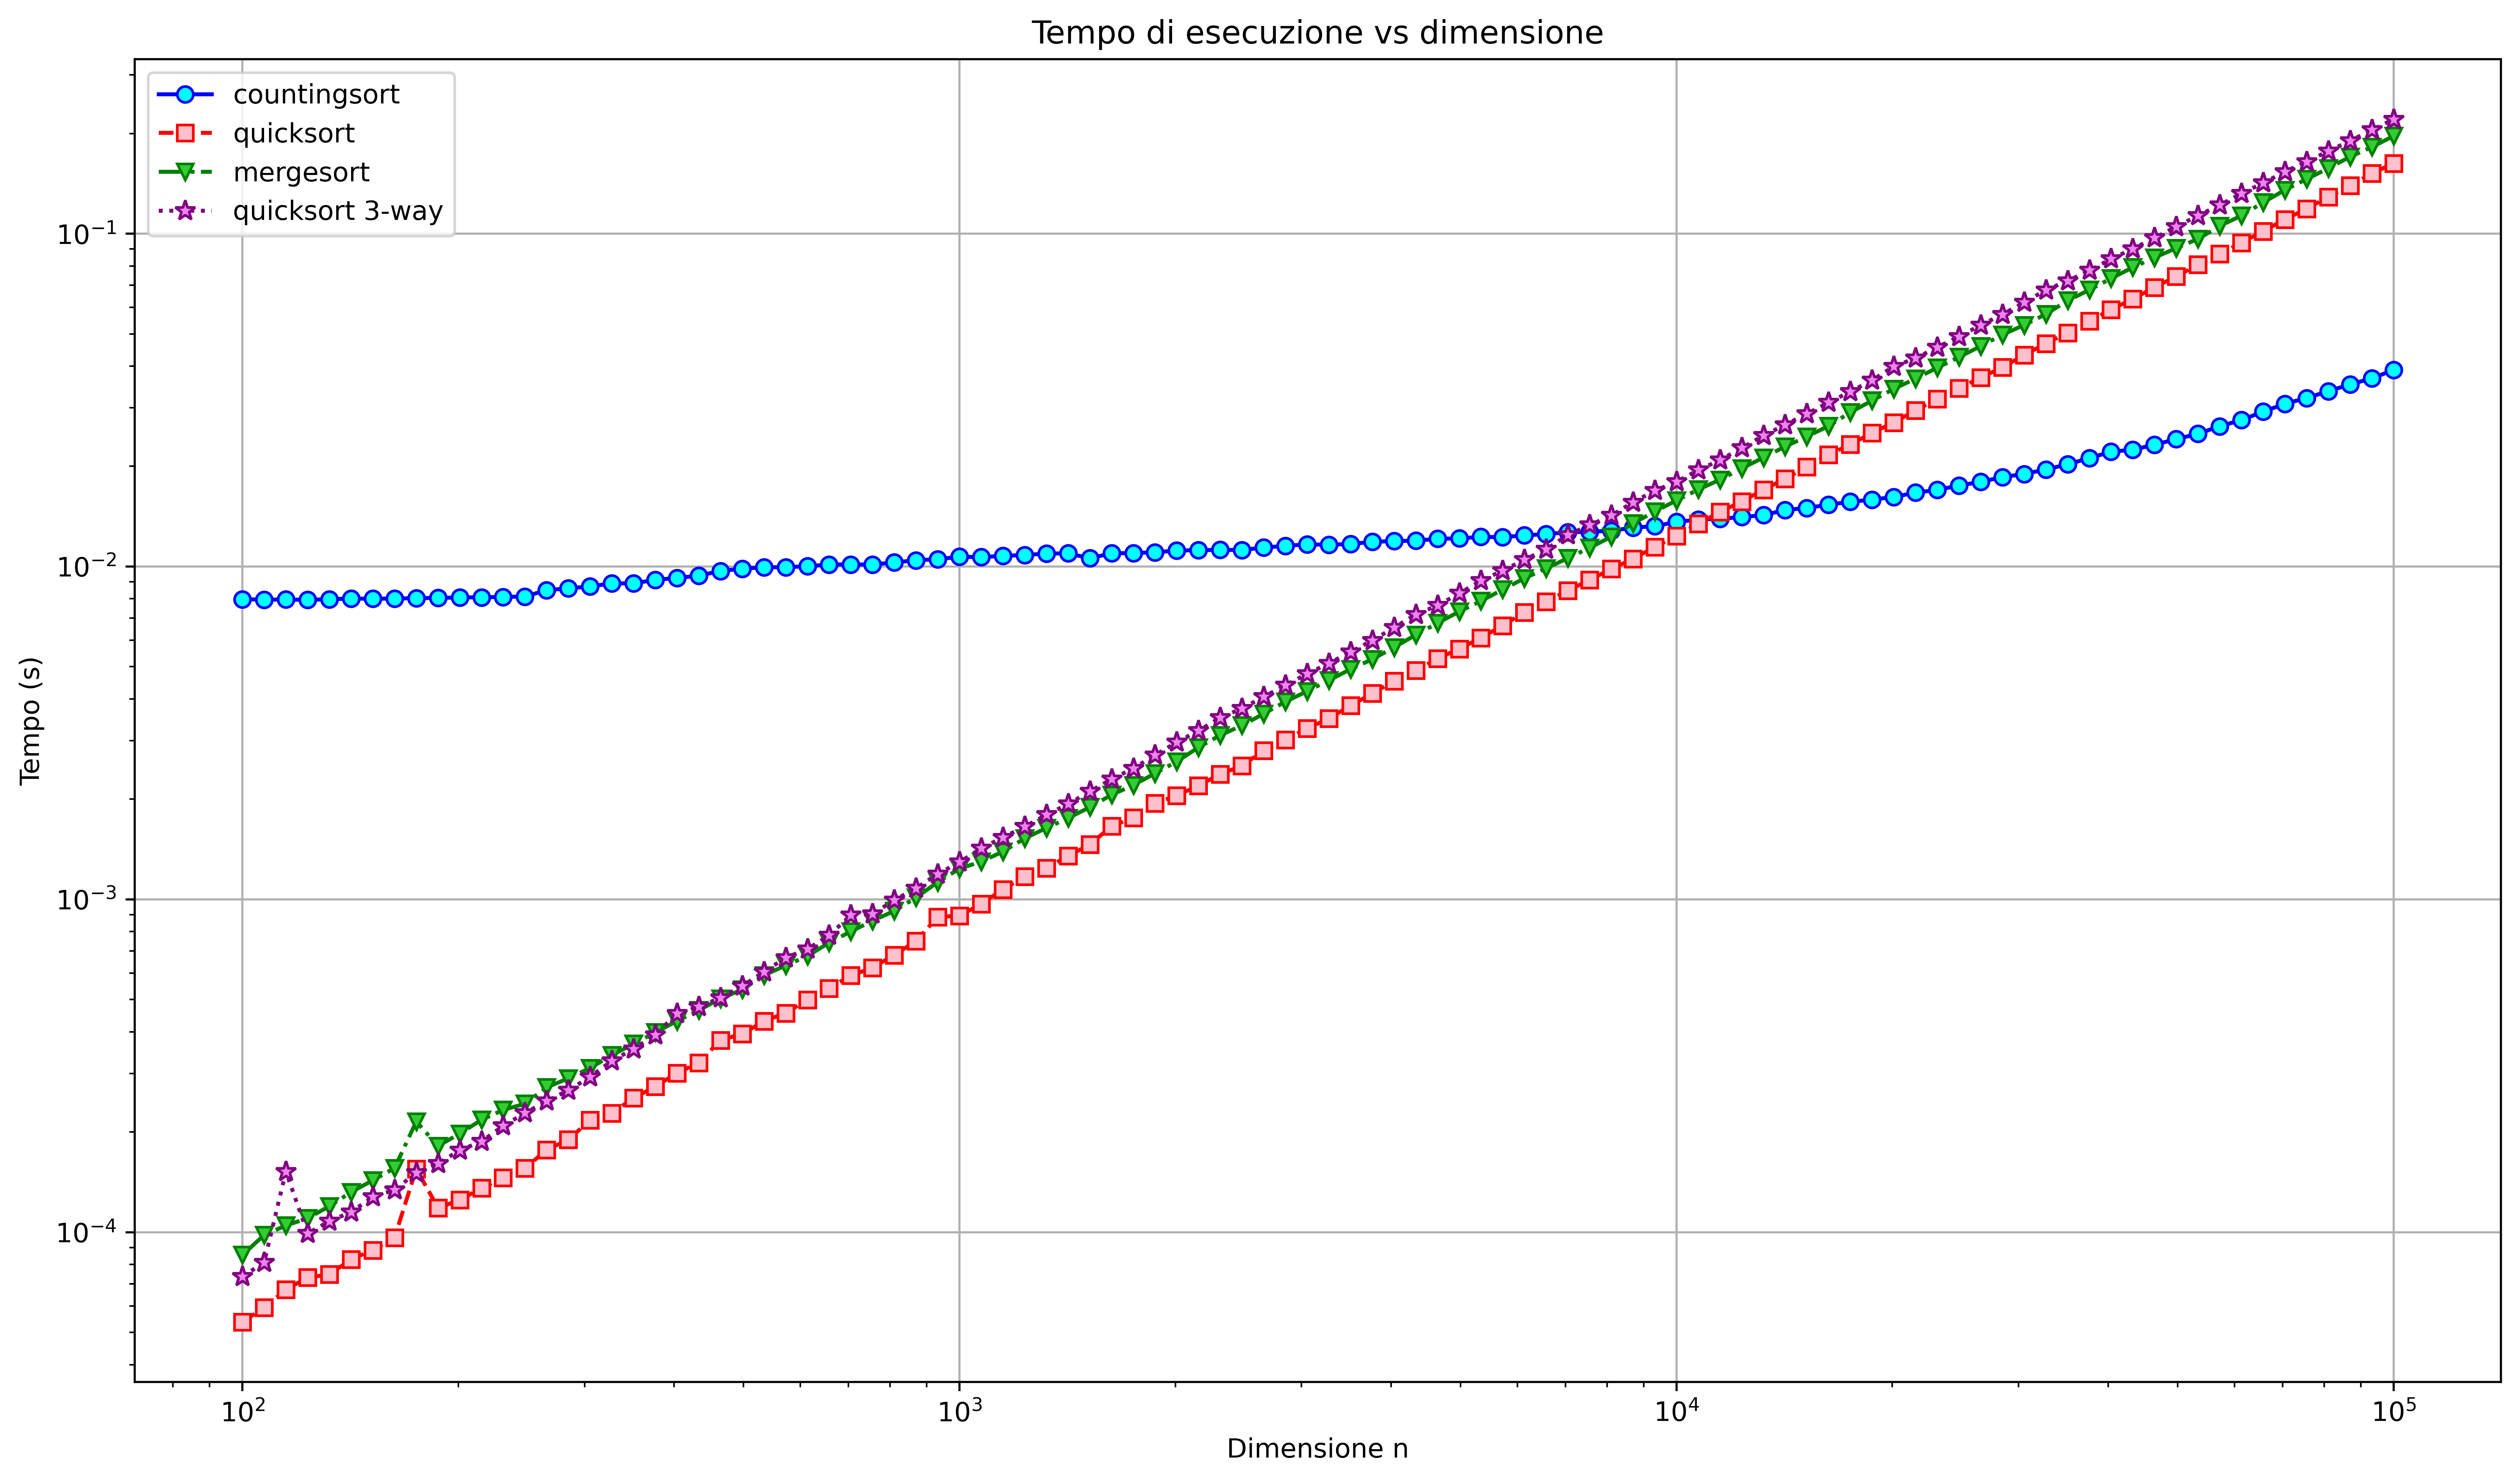
\includegraphics[width=0.95\textwidth]{Casi medi/nlog.png}
    \caption{Graph in double logarithmic scale as a function of array size \emph{n}}
    \label{fig:nlog}
\end{figure}

From the graph \emph{[Fig. 1]}, it can be observed that the x-axis shows an increasing array size \emph{n}, while the range of integers is fixed at $10^5$ elements. The y-axis displays the execution time \emph{t} of the algorithms for sorting the array.

It is evident that Countingsort is \textbf{slower} than the other algorithms when working with arrays of smaller magnitudes. As the array size increases, Countingsort becomes notably faster (from the order of magnitude $n = 10^4$ onwards).

This change is explained by the fact that, since the array consists of integers taken from a fixed range of values, as dimension \emph{n} increases, the number of \textbf{repeated elements} also grows. In this circumstance, Countingsort excels due to its structure. Furthermore, its computational complexity is lower than the other algorithms: $O(n + k)$. Since $k \approx m$ is fixed a priori, as dimension increases, the complexity of the other three algorithms, $O(n \log(n))$, makes execution times less advantageous compared to Countingsort.

The other three compared algorithms (Mergesort, Quicksort, and Quicksort 3-way) show similar performance among themselves, as they share the \textbf{same average computational complexity} of $O(n \log(n))$.

In the double logarithmic scale graph \emph{[Fig. 2]}, the performance difference is much more evident as the order of magnitude of array size \emph{n} varies:
\begin{itemize}
    \item for $n \leq 10^4$: Countingsort is much less efficient than the other algorithms
    \item for $n > 10^4$: Countingsort becomes the most efficient
\end{itemize}
The double logarithmic scale allows us to evaluate for each \textbf{order of magnitude} of dimension \emph{n} which algorithm is most efficient.

\subsection*{Variable Range}

\begin{figure}[H]
    \centering
    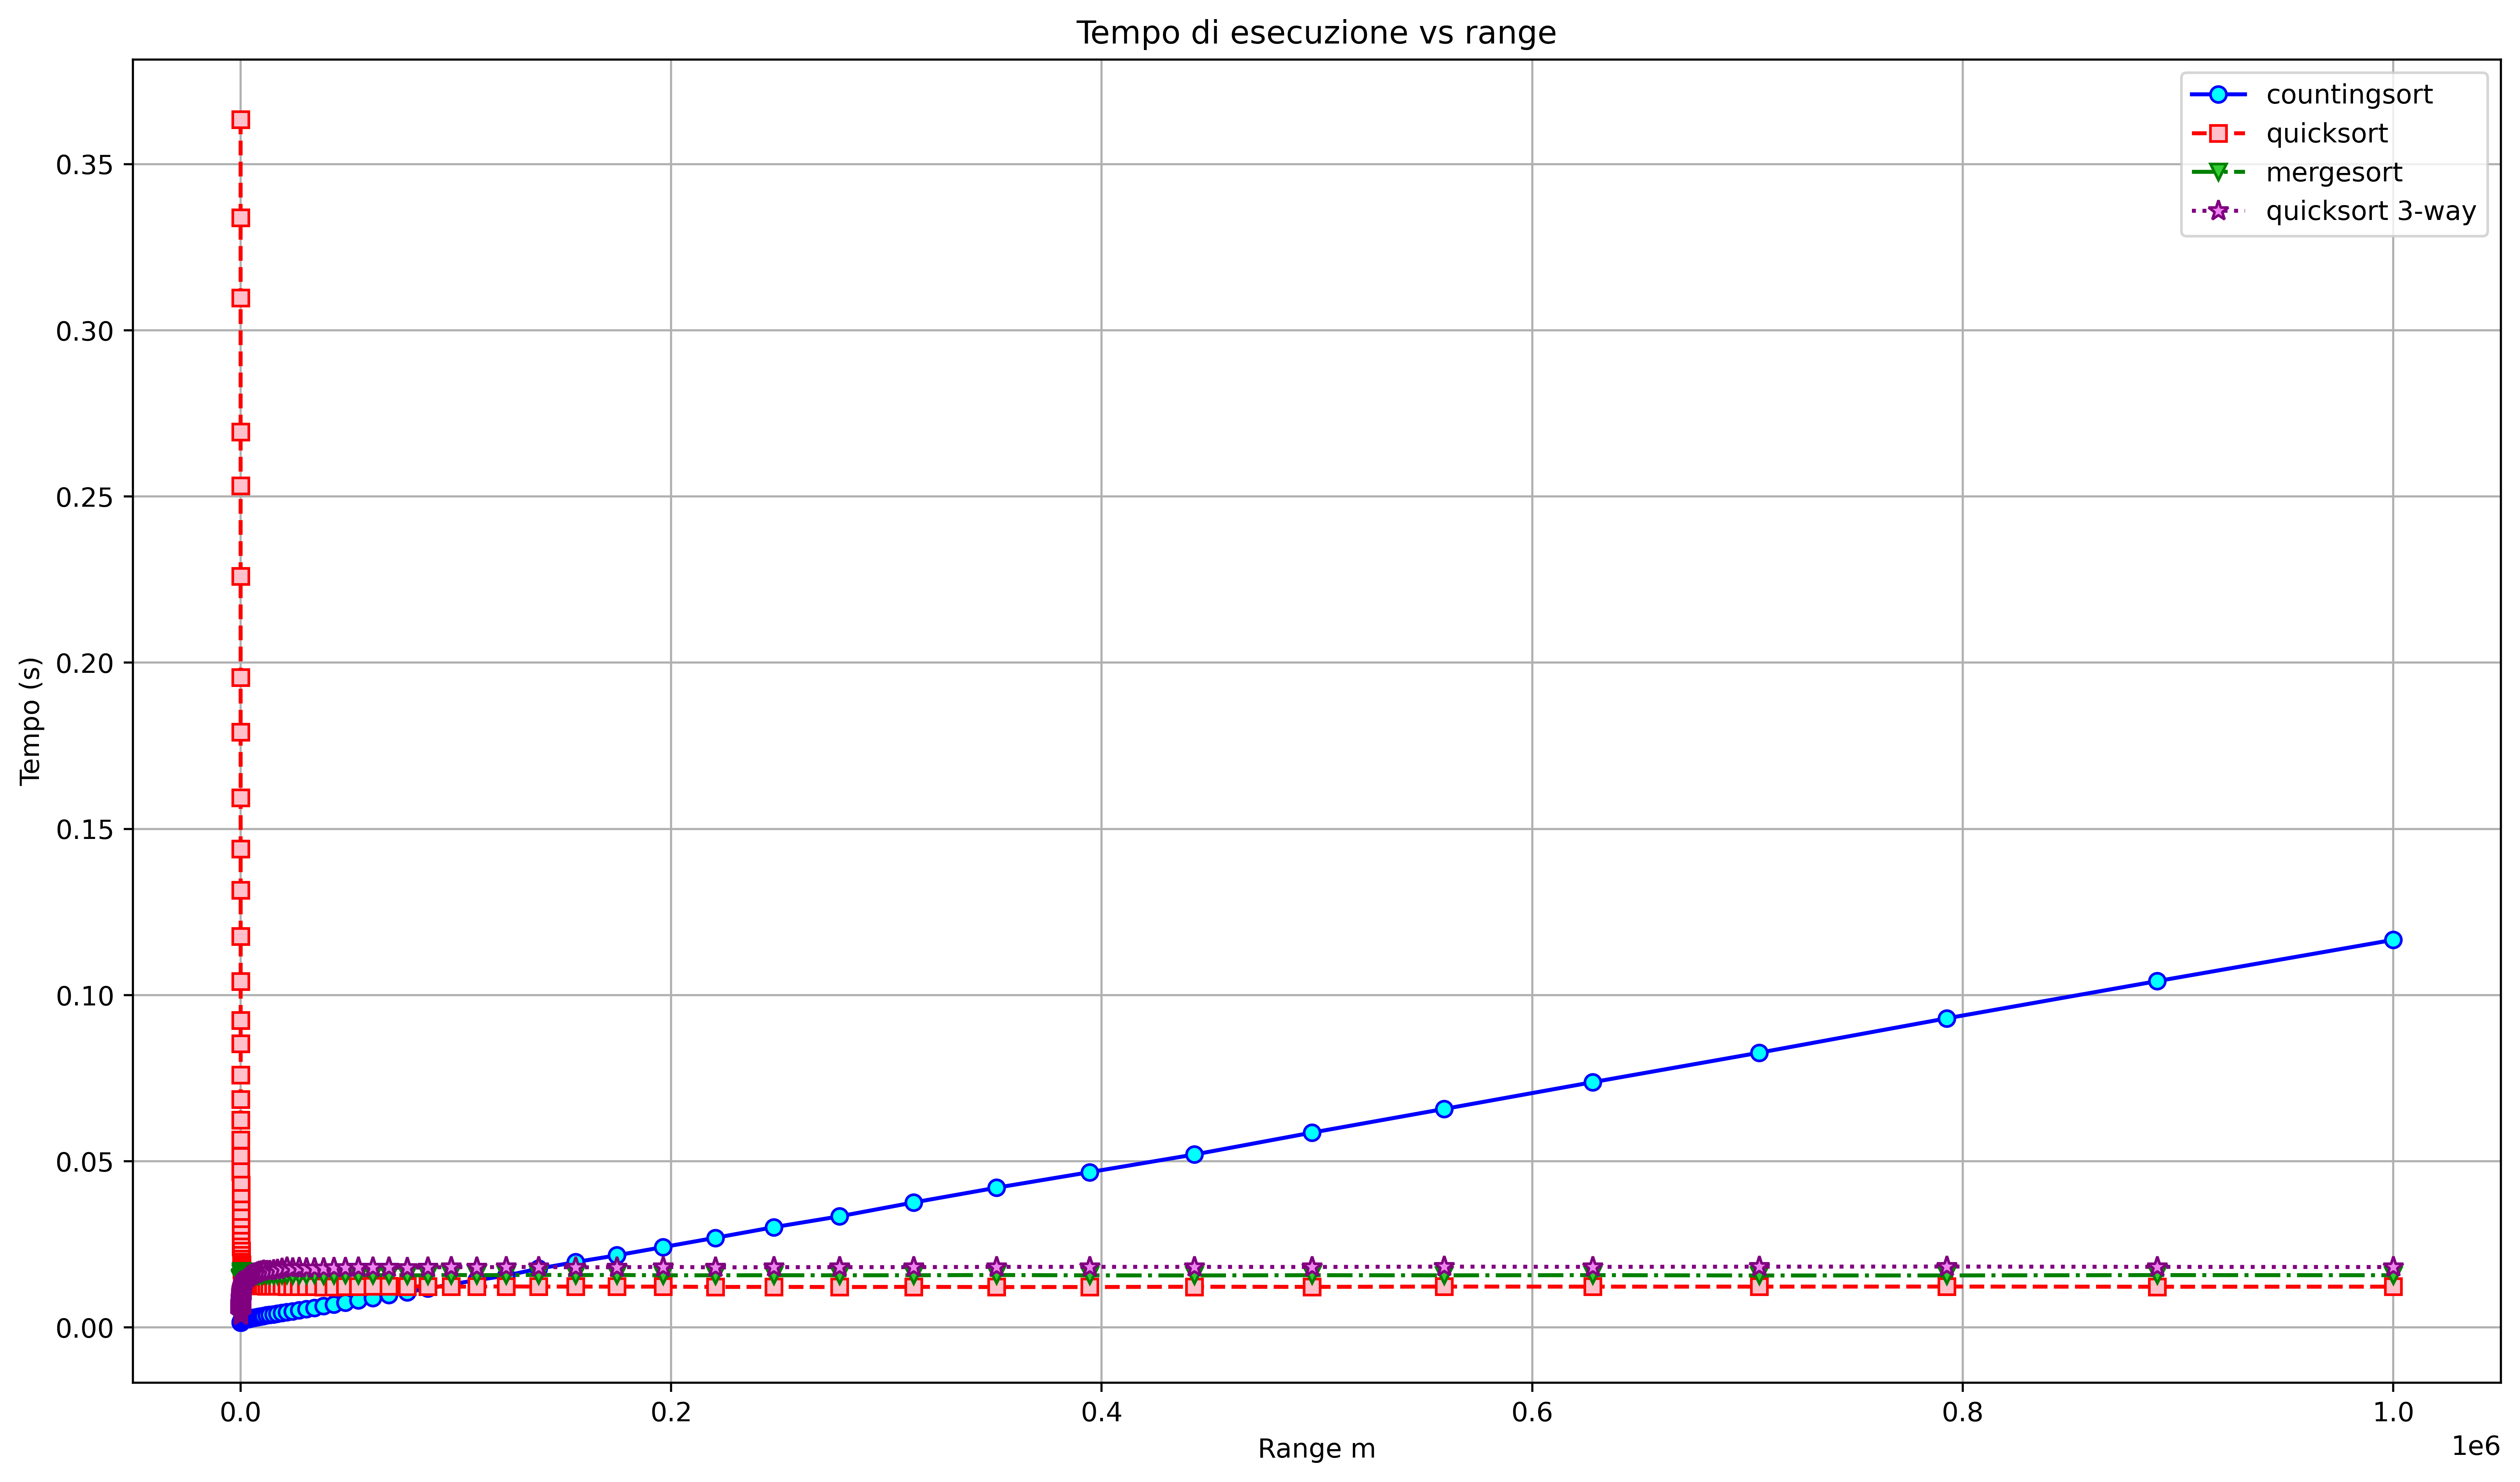
\includegraphics[width=1\textwidth]{Casi medi/m.png}
    \caption{Graph as a function of the range of integers \emph{m}}
    \label{fig:m}
\end{figure}

The graph \emph{[Fig. 3]} shows the execution times of the sorting algorithms as the range \emph{m} of integers composing the arrays varies. The sample arrays have a fixed size \emph{n} of $10^5$ elements.

When the range of integers becomes wider, Countingsort is the \textbf{least efficient} algorithm, since it must store a \textbf{larger number of values}. From the linear graph we observe that:
with small ranges, classical Quicksort is the slowest while Countingsort is the fastest.

\begin{figure}[H]
    \centering
    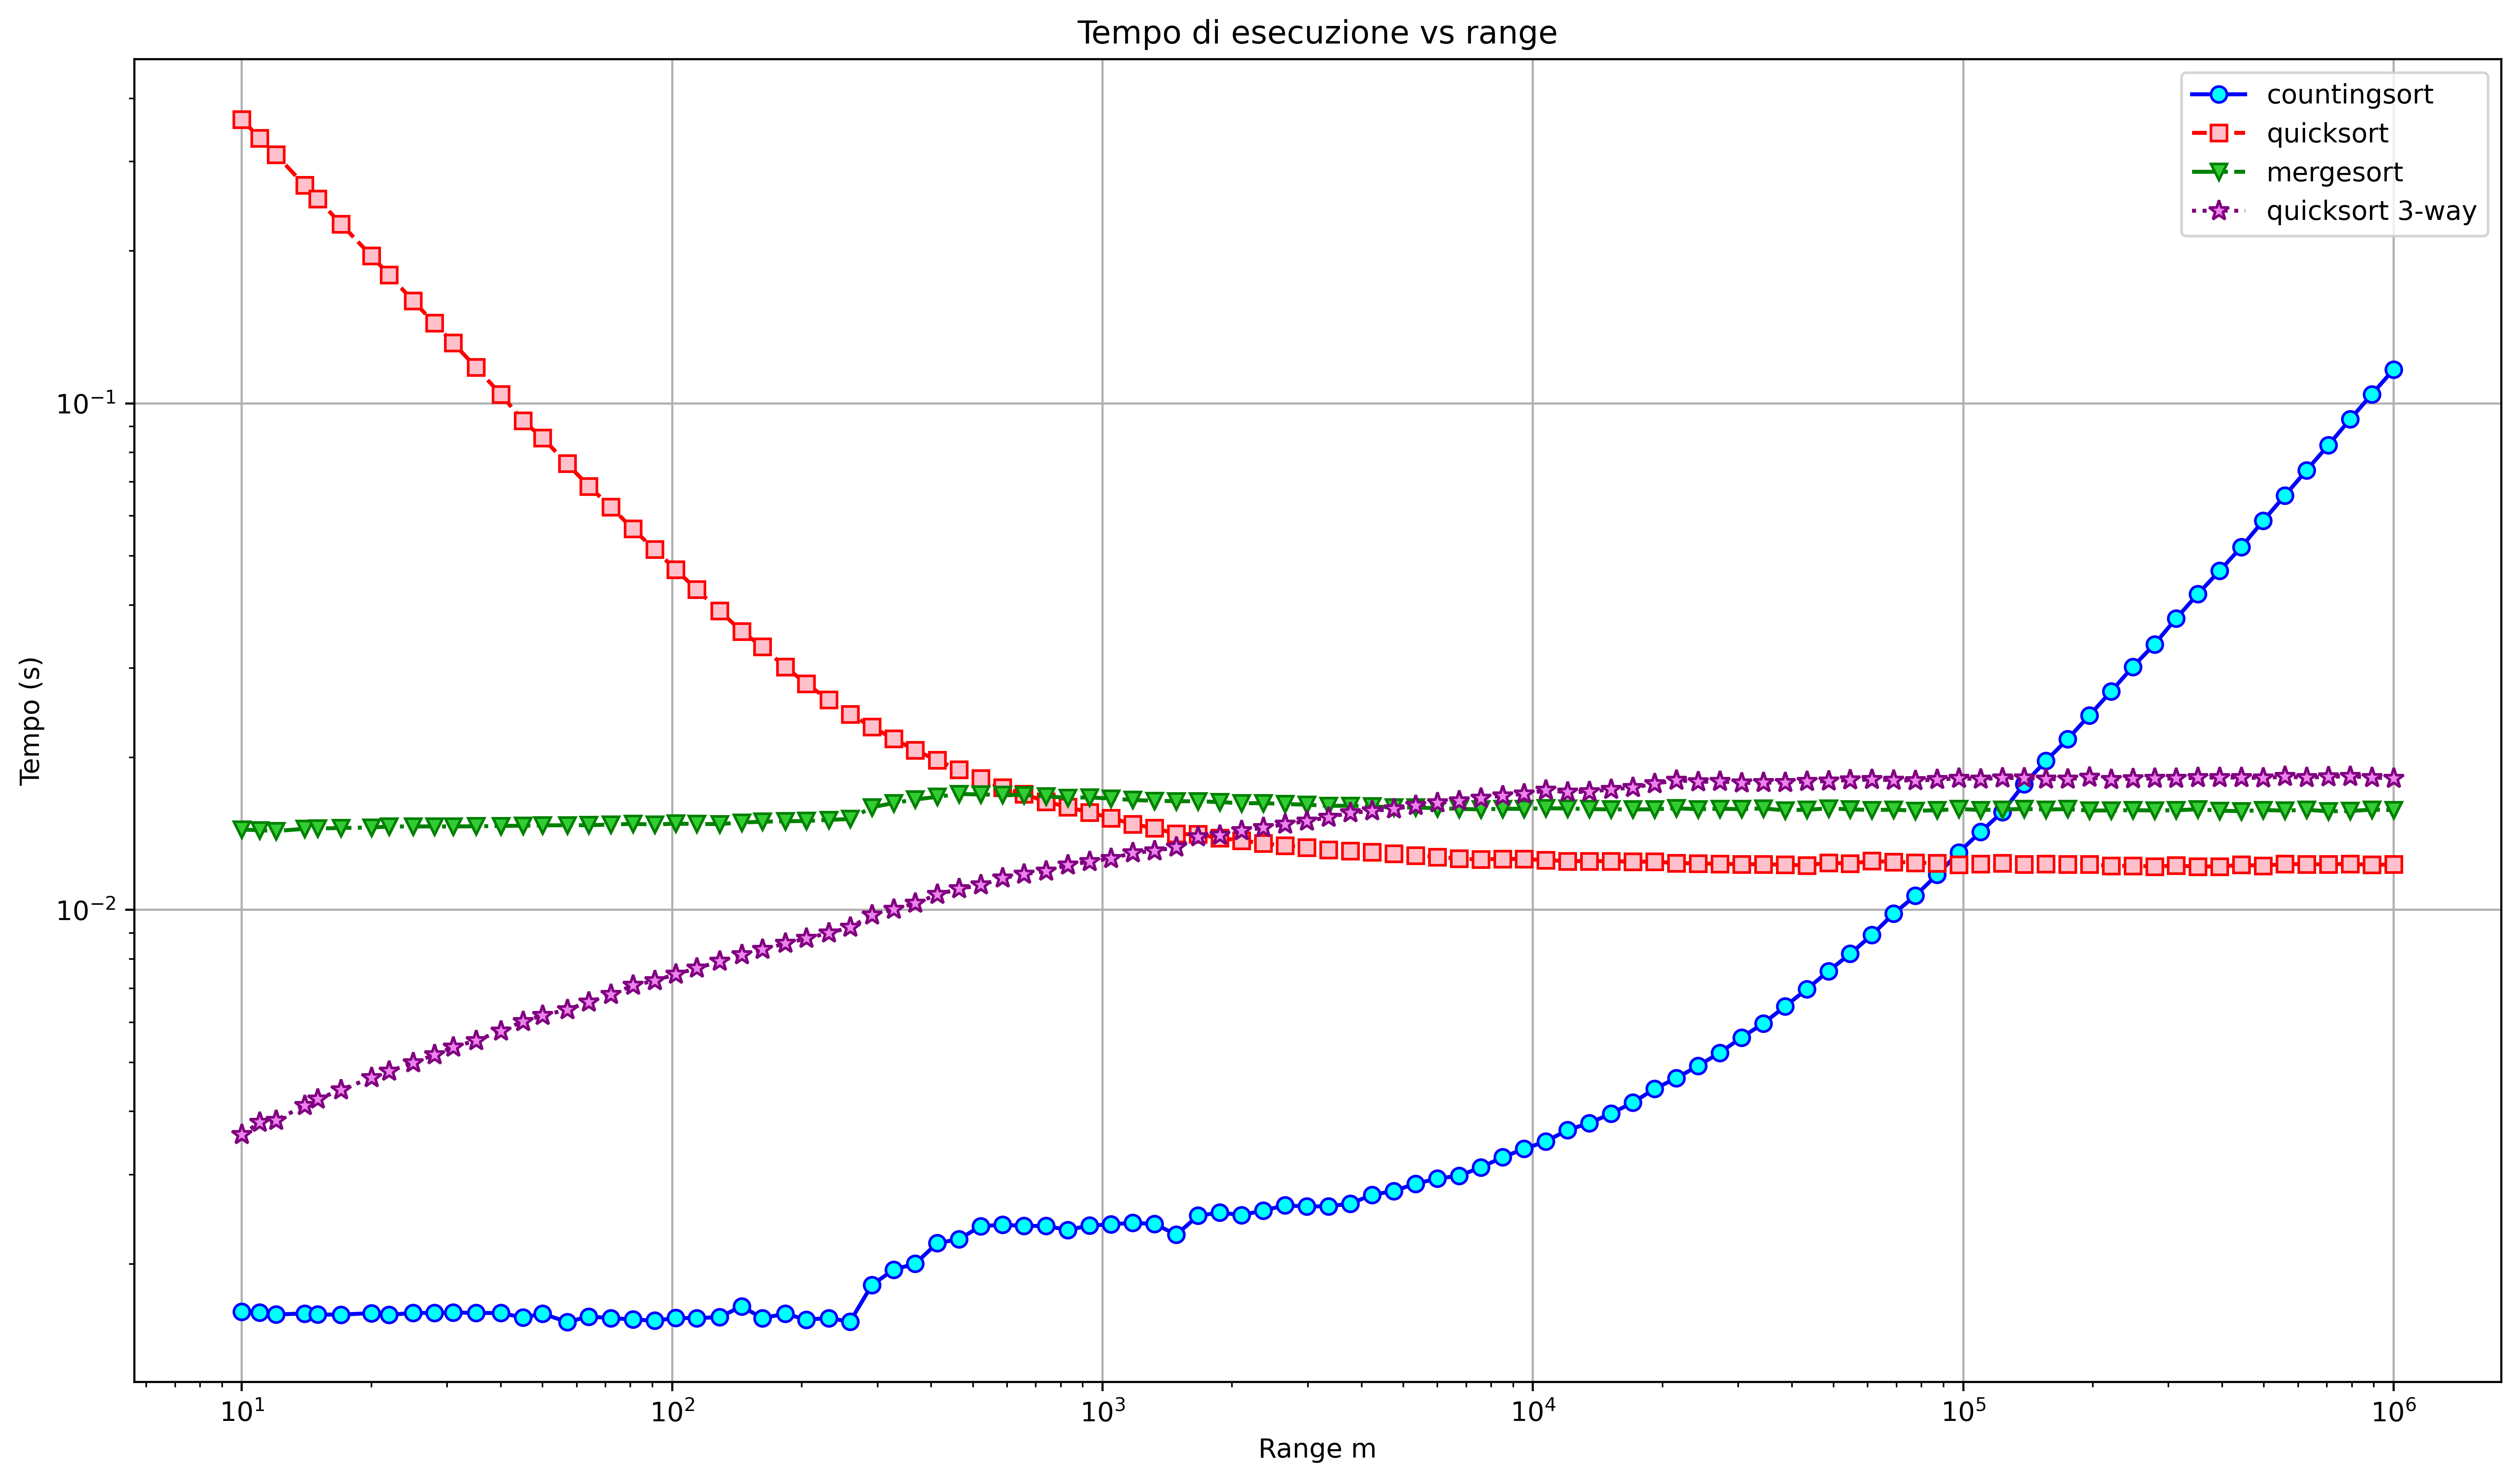
\includegraphics[width=1\textwidth]{Casi medi/mlog.png}
    \caption{Graph in double logarithmic scale as a function of the range of integers \emph{m}}
    \label{fig:mlog}
\end{figure}

In the graph \emph{[Fig.4]} in double logarithmic scale, the trend is clearer:
With range $m < 10^3$ classical Quicksort is the least efficient, since the presence of \textbf{many repeated values}, typical of narrow ranges, penalizes its performance. Quicksort 3-way is instead optimal in comparison, thanks to its ability to efficiently handle repeated values, a problem that disappears as the evaluated range increases.

Similarly, Countingsort performs better with small ranges, with execution times lower than other algorithms. This happens because Countingsort does not perform comparisons between array elements, but counts the \textbf{occurrence} of each value.

When the order of magnitude exceeds $10^3$, the execution times of the two Quicksort versions and Mergesort become stable, since the number of repeated elements in an array becomes \textbf{negligible}.

With range $m > 10^5$ Countingsort becomes the slowest, since the growth of the range increases the storage cost.
The other algorithms (Mergesort, Quicksort, Quicksort 3-way) show similar execution times.

Mergesort maintains a \textbf{constant} execution time as the range \emph{m} increases. This algorithm is not influenced by the presence of repeated values since it does not use pivots and does not create structures tied to the maximum and minimum values present in the array. It works only as a function of the array size.

\section{Analysis of Graphs in Worst Case Scenarios}
\label{sec:peggiori}

\subsection*{Worst Case Generation}

To analyze worst cases, an array was generated with unique values inserted in descending order. For Countingsort, we chose to fix the maximum and minimum values in order to obtain an array with the maximum possible range. This choice stems from the fact that the worst case for Countingsort occurs when the array contains all different elements distributed over a wide range of values: in this case, the algorithm is forced to allocate significant memory to handle each value individually. As for Mergesort, we generated an array using a method called \textbf{perfect alternation}, in which the sequence of elements is generated such that each half has interleaved elements, that is, large and small elements alternate, and the algorithm is forced to compare every single element.

\subsection*{Graphs}

\begin{figure}[H]
    \centering
    
\includegraphics[width=1\textwidth]{Casi peggiori/n.png}
    \caption{Graph in linear scale of worst cases as a function of size \emph{n}}
    \label{fig:npeggiori}
\end{figure}

From the linear graph \emph{[Fig. 5]} it is noted that the slowest algorithms are Quicksort and Quicksort 3-way, since they have worst-case complexity equal to $O(n^2)$. Quicksort 3-way, by performing a greater number of comparisons, is much slower on large arrays, especially when there are no duplicate elements and the elements are ordered in descending order.
Regarding Countingsort and Mergesort, from the linear graph we cannot make a detailed evaluation because their curves are overlapped and are in any case much faster than the other two algorithms.

\begin{figure}[H]
    \centering
    
\includegraphics[width=1\textwidth]{Casi peggiori/nlog.png}
    \caption{Graph in double logarithmic scale of worst cases as a function of size \emph{n}}
    \label{fig:nlogpeggiori}
\end{figure}

To better analyze the behaviors, we move to the double logarithmic scale \emph{[Fig. 6]}, from which we observe that Countingsort grows very slowly as the size increases, but in the initial phases, on small arrays, it is the least efficient algorithm.

We note that two algorithms do not change behavior:
\begin{itemize}
\item Mergesort, having complexity $O(n \log(n))$, shows moderate growth. Comparing it with its average cases \emph{[Fig. 2]}, it achieves \textbf{the same performance}. This happens because Mergesort divides the array in the same way into subvectors regardless of the values it contains.
\item Countingsort does not change behavior compared to the average case \emph{[Fig. 2]}. This can be explained by the fact that in the average case, arrays were generated with a very wide range. Because of this, in the average case it is equally difficult to find many repeated values. The worst case for Countingsort occurs when the range \emph{m} of integers is much larger than the size of the array to be sorted. It is \textbf{not sensitive} to the initial arrangement of the array.
\end{itemize}
\newpage
\section{Project Contributors}
\label{sec:partecipanti}
Federico Del Pup  \\
Matteo Passador    \\
Luigi Pascu       \\
Stefano Toneguzzo \\




\end{document}
